\documentclass[a4paper,twoside,10pt]{report}
%picture imports
\usepackage{graphicx}
\usepackage{color}
\usepackage{fancyhdr}
\definecolor{lbcolor}{rgb}{0.85,0.85,0.85}

%sourcecode formatting
\usepackage[final]{listings}
\usepackage{url}


\lstloadlanguages{Eiffel,bash,Java}
\newcommand{\eiffellisting}{\lstset{basicstyle=\small,language=Eiffel,tabsize=2,backgroundcolor=\color{lbcolor},frame=tb,breaklines=true}}
\newcommand{\bashlisting}{\lstset{basicstyle=\small\tt,language=bash,tabsize=2,backgroundcolor=\color{lbcolor},frame=tb,breaklines=true,morekeywords={svn,geant,mkdir,activate_estudio}}}
\newcommand{\javalisting}{\lstset{basicstyle=\small,language=Java,tabsize=2,backgroundcolor=\color{lbcolor},frame=tb,breaklines=true}}
\newcommand{\identifier}[1]{\texttt{#1}}
\newcommand{\figref}[1]{Figure \ref{#1}}
\newcommand {\class}[1] {\texttt{#1}}
\pagenumbering{roman}

\begin{document}

%opening
\title{Selective Capture and Replay for Eiffel}
\author{Stefan Sieber}

\begin{titlepage}
	\begin{flushleft}
		
\includegraphics[width=100pt]{illustrations/SE.png}
	\end{flushleft}

	\vskip 50pt
	\begin{center}
		\Huge \textbf{Capture and Replay for Eiffel}
	\end{center}

	\vskip 100pt
	\begin{flushright}
		\large \textbf{Stefan Sieber}\\
		\vskip 10pt
		02-911-790\\
		Master Thesis\\
		Summer 2007\\
	\end{flushright}
	
	\vskip 20pt
	\begin{flushright}
		\large Chair of Software Engineering\\
		Department of Computer Science\\
		ETH Z\"{u}rich
	\end{flushright}
		
	\vskip 20pt
	\begin{flushright}
		\large Andreas Leitner\\
		Prof. Bertrand Meyer
	\end{flushright}

	\vskip 50pt
	\begin{tabular*}{1.00\textwidth}{@{\extracolsep{\fill}}lr}
		 
\includegraphics[width=100pt]{illustrations/ETH.png} &
		 
\includegraphics[width=100pt]{illustrations/INF.png}
	\end{tabular*}
	\vfil
\end{titlepage}

%prolog
\addtolength{\parskip}{0.5\baselineskip} % add extra spacing between paragraphs
\newpage
\pagenumbering{roman}
\section*{Abstract}

ABEL is an approach to wrap every existing persistence library under a simple and yet powerful API.
The programming interface of ABEL is completely transparent to the actual storage mechanism, and it supports the CRUD operations, transactions, and some advanced features like result filtering based on some criteria.

ABEL has a flexible framework that allows to adapt the API to basically any existing persistence solution.
The framework has a reusable object-relational mapper at its core and is open for extensions and customization.

% table of contents
\addtolength{\parskip}{-0.5\baselineskip} % reset paragraph spacing
\tableofcontents

\newpage

% chapters
\pagenumbering{arabic}
%configure headers:
\pagestyle{fancy}%
\renewcommand{\headrulewidth}{0.3pt}
\renewcommand{\footrulewidth}{0pt}
\renewcommand{\chaptermark}[1]{\markboth{\MakeUppercase{#1}}{}}
\renewcommand{\sectionmark}[1]{\markright{\MakeUppercase{#1}}{}}
\fancyhf{}
\fancyhead[LE,RO]{\thepage}
\fancyhead[LO]{\rightmark}
\fancyhead[RE]{\leftmark}
\fancyfoot{}

\addtolength{\parskip}{0.5\baselineskip} % add extra spacing between paragraphs
\section{Introduction}

The Eiffel language \cite{EcmaEiffel} \cite{Meyer09} has a lot of different persistence libraries, and every solution has its own advantages and drawbacks.
A database such as MySQL \cite {MySQL} for example is quite fast, but it comes at the expense of the object-relational impedance mismatch \cite{ORImpedance}.
A serialization library on the other hand is easier to handle for the programmer, but its performance rapidly decreases for large data sets.

It is very hard to switch from one persistence solution to another, because all have their own interface.
Even changing for example the data\-base from MySQL to Oracle \cite{Oracle} is usually very hard to achieve, if only because their SQL dialects are different.

To overcome such problems we have developed a new library called ABEL, which is the acronym for ``A better Eiffelstore library''.
ABEL tries to unify existing persistence libraries unter a simple and yet powerful API, which is completely transparent to the actual storage mechanism.


\section{Overview}
This thesis is basically splitted into two parts: The API tutorial and the technical documentation.

In the first part you will be introduced to the basic operations of the API, like the CRUD (Create, Read, Update, Delete) operations or transaction handling.

The second part is an introduction to the general architecture of ABEL and some selected topics like the object-relational mapping layer or the main interfaces for backend abstraction.

\chapter{Related Work}
%TODO: kurze einleitung

\section{Overview}
Because replaying application runs is important in order to be able to debug or test applications, there exist many techniques that implement capture and replay. One of the basic steps in order to be able to capture and replay an application is to distinct between the applications deterministic core (the \emph{observed part}) and the non-deterministic environment like user input, network or external storage (the \emph{unobserved part}). Capture and replay techniques capture the interactions between observed and unobserved part during \emph{capture phase} so that they can replay these interactions on the observed part during the \emph{replay phase}.

% -------
% Dieser Teil koennte sonst noch irgendwo untergebracht werden.
%--------
% In general, capture and replay can be divided into two phases: The \emph{capture phase}, where the application is run and the information that is needed for replaying the application is captured and the \emph{replay phase} where the application is replayed based on this information.
% 
% During \emph{capture phase}, the capture and replay implementation needs to record the information that will later be needed to replay the observed part. In general this is at least all information that is passed from the unobserved part to the observed part. The information is captured by some management code that was introduced by the capture and replay framework (\figref{fig:GenericCrStructure_capture}).

% 
% During \emph{replay phase} the management code needs to replace the unobserved part ( 
% \figref{fig:GenericCrStructure_replay}) in order to replay the run of the observed part. Depending on the part of the application that was defined to be unobserved, the management part can act both as a driver (e.g. in the case of mouse events) and stub (e.g. in the case of a network socket). 
% %Schema dazu: Capture phase & Replay phase , observed & unobserved part && log
% \begin{figure}[h]
%   \centering
%   \includegraphics[width=0.4\textwidth]{illustrations/capture_and_replay_generic_structure_replay}
%   \caption{Generic structure of a capture and replay technique - replay phase}
%   \label{fig:GenericCrStructure_replay}
% %\includegraphics{illustrations/capture_and_replay_generic_structure}
% \end{figure}

Different implementations make different assumptions about what is deterministic and what changes its behaviour throughout different runs of the application. Therefore they define different portions of the program as observed and unobserved part. In the following we will categorize the different implementation based on which part is defined to be unobserved.

\section {Capturing User Input}
The best known capture and replay technique is the capturing of user input, which is most often used for GUI testing. Here, keyboard and mouse events are considered to come from the unobserved part. The exact location where these events are captured may vary (inside the application or through the operating system), but the advantages and limitations mostly stay the same. Usually, capture and replay of user input is used for regression testing. In that setup, the tester executes a sequence of actions on the applications GUI while capturing is enabled. These recorded actions can be replayed on the application in order to check if there were regressions. Abbot \cite{abbot} is an example of such a tool, although it offers more features than only capture and replay of user interactions. %TODO: wie funktioniert Abbot?

Compared to our implementation, the capturing of user inputs has many drawbacks due to its simplicity. Because only the user input is considered to belong to the unobserved part, it can replay programs that interact with other parts of the environment (like file system and network) only as long as these interactions are deterministic. One strategy is to restore the environment before every run of the application, but this is not always easy (e.g. if a random generator is used). If the assumption, that the observed space behaves deterministically does not hold, this results in an incorrect replay of the application. Because our implementation makes it possible to individually define the applications observed and unobserved part, it can also replay programs that depend on other parts of the non-deterministic environment than only the user input.

\section {Capturing Interactions with Libraries}
JRapture \cite{jrapture} uses an approach that has the potential of replaying more complex applications. JRapture is a tool for capturing and replaying Java applications in the field. In addition to capturing and replaying, it also offers a profiling interface that permits the program to be instrumented for profiling in the replay phase. JRapture uses the whole Java API api as the unobserved part of the application. The technique is able to capture interaction between the Java API and the rest of the program by manual instrumentation of the Java API classes. JRapture supports multithreaded applications, but it can not guarantee a deterministic replay of concurrent applications.

Unlike our technique, JRapture relies on a manually modified version of libraries. Programs that need to be captured and replayed need to use a special version of the Java API.  This results in the fact that programs that interact with the environment through other mechanisms than the Java API (for example through the Java Native Interface JNI) can not be supported without additional manual instrumentations.

%genauer veranschaulichen, was complete und incomplete ist.
JRapture captures the complete information that is passed between the observed and unobserved part, in contrast to our approach that only captures necessary information.

\section {Capturing Interactions with the Scheduler}
The techniques presented so far did not consider thread scheduling as another source of non-determinism. DejaVu \cite{dejavu}, a capture and replay tool for Java, considers thread scheduling as its only source of non-determinism, thus thread scheduling belongs to its unobserved part. It is not easy to instrument the scheduler in order to detect thread switches, because threads are often scheduled by the operating system. DejaVu therefore introduces the concept of \emph{logical thread schedule} which is a simplified version of the real thread schedule (the \emph{physical thread schedule}). The \emph{logical thread schedule} contains enough thread schedule information to reproduce the execution behaviour of the program under the assumption that the thread schedule is the only source of non-determinism. By detecting some critical events during capture phase such as accesses to shared variables, and synchronization events, DejaVu is able to deduce the logical thread schedule.

DejaVu concentrates on enabling a determistic replay of multi threaded programs that do not have any other source of non-determinism than the thread scheduler. Our technique does not take the non-determinism of the thread scheduler into account, instead it concentrates on all other interactions with the environment. DejaVu and 
%TODO referenz auf Orso.
our technique are orthogonal and could be combined in order to allow replays of general concurrent programs. 

\section{Selective Capture Replay}
In contrast to other techniques, \emph{selective capture and replay} \cite{orso05may} implemented for Java, offers the user the possibility to make his own definition of observed and unobserved part of the system.
%TODO 2x passiv!
Observed and unobserved part are both defined as a set of classes. The interactions between observed and unobserved part are captured using automated code instrumentation.

%TODO: 2 verschiedene implementierungen (???) Zeller vs. Orso

Our work tries to transfer the concept from the original paper \cite{orso05may} to Eiffel Our implementation instruments code in a different way and adds some Eiffel specific modifications.
%TODO: zwei 


\chapter{Preleminaries}
In this section we will first present an example application that will be used throughout the report. Then, the paper about the original implementation of selective capture and replay by Joshi and Orso \cite{orso05may} will be summarized.


\section{Example Application}
In the following we will present our example application. It will be explained in detail here and then be used throughout this report.

Consider a customer that wants to withdraw money from his account. He interacts with the user interface at an ATM (\figref{fig:example_class_diagram}). This user interface could be implemented in different ways (textual or graphical). The transactions that the customer executes at the user interface are first written to the ATM's journal and then dispatched to the bank. When the customer wants to withdraw money, the bank withdraws money from the customers bank account and the ATM then hands the money to the customer.
 \begin{figure}[ht]
   \centering
   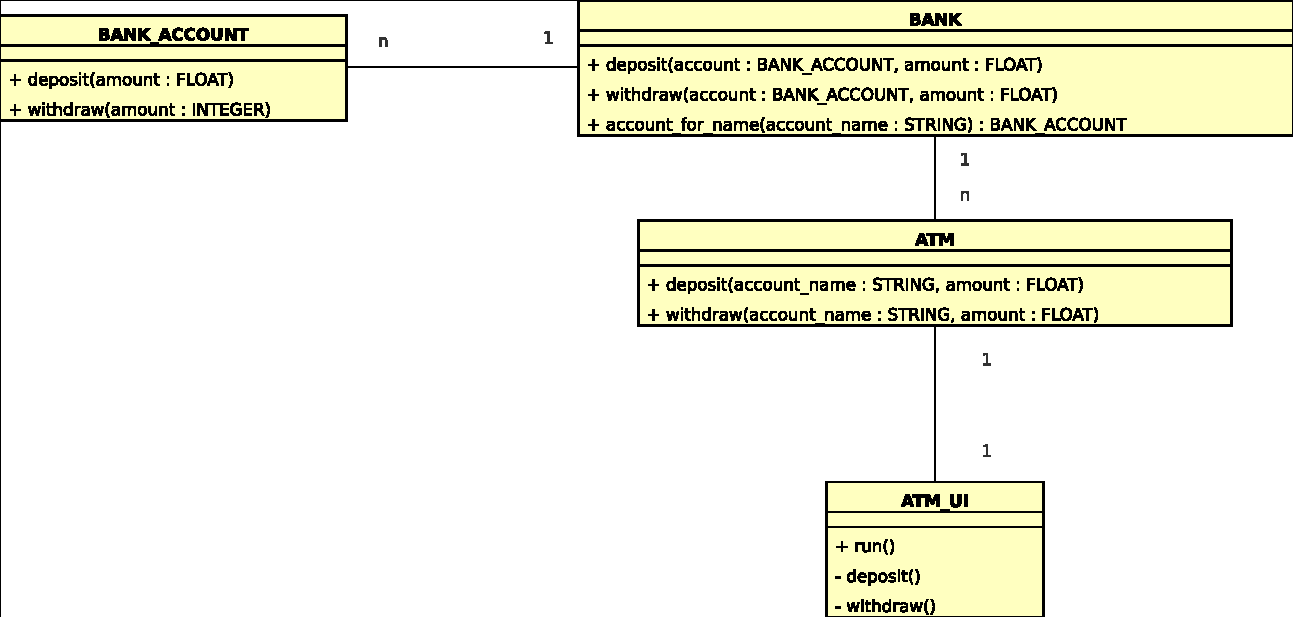
\includegraphics[width=1\textwidth]{illustrations/example_class_diagram}
   \caption{Class Diagram showing the example of a Bank and ATMs}
   \label{fig:example_class_diagram}
\end{figure}

Note that the names of classes and methods were apply to the style presented in Object Oriented Software Construction, second edition \cite{oosc2}. Even Java examples that refer to this application will use that style to keep the same class and method names.

\begin{figure}[ht]
   \centering
   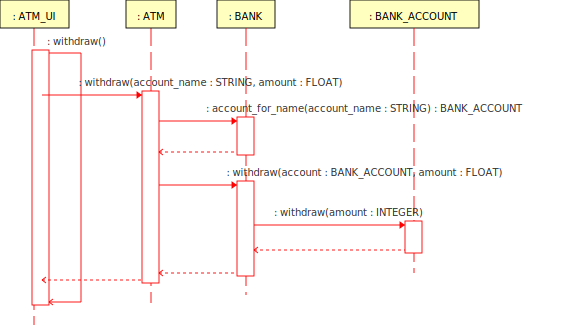
\includegraphics[width=1\textwidth]{illustrations/example_withdrawal}
   \caption{Sequence Diagram of a Withdrawal Operation Invoked by the Customer}
   \label{fig:example_withdraw_sequence}
\end{figure}

One use case is money withdrawal by a customer via an ATM. The customer launches the withdrawal operation on the ATM\_UI. The request is passed through the ATM to the BANK which then withdraws the money from the Account. The sequence diagram (\figref{fig:example_withdraw_sequence}) should clarify how the classes interact with each other.



\section{Selective Capture and Replay}
After giving the overview about the different capture and replay techniques in the related work chapter	, our choice will be described here in detail. Currently there exist two implementations of selective capture and replay, both for Java: SCARPE \cite{orso05may, orso06}, the original implementation, and JINSI \cite{JINSI}, which minimizes failure inducing component interactions that were captured using selective capture and replay.

This chapter summarizes papers from Joshi and Orso about original implementation of selective capture and replay (SCARPE) \cite{orso05may, orso06}. Where appropriate, some examples using the application described before are introduced.

\subsection{Technique and Terminology}

\begin{figure}[ht]
  \centering
  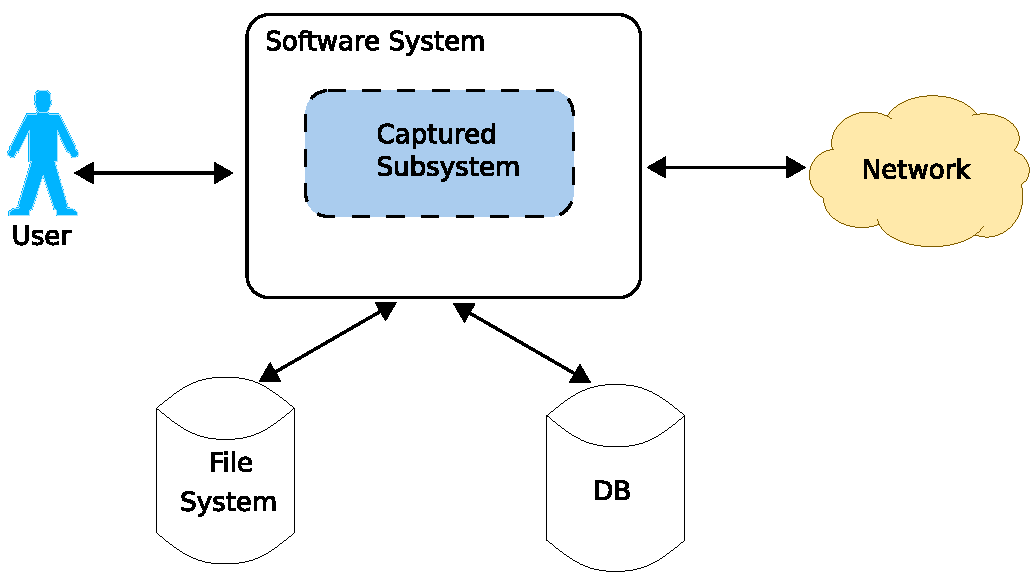
\includegraphics[width=1\textwidth]{illustrations/scr_overall_schema}
  \caption{System Layout of the Example Application Showing the Captured Subsystem (derived from Joshi and Orso \cite{orso05may})}
  \label{fig:scr_overall_schema}
\end{figure}

This technique lets the user choose the subset of the program that should be captured and replayed (\emph{captured subsystem}, \figref{fig:scr_overall_schema}). It then only captures the execution data of that subsystem, ignoring the other parts of the system. The relevant interactions between the captured subsystem and the outside world is captured in terms of events; those events are read during the replay phase in order to replay the corresponding interactions. Only the essential part of the information that traverses the border between the captured subsystem and the rest of the system is captured. This is a significant improvement over other existing techniques that capture all the data, especially when big datastructures are passed over the border and only a part of those datastructures is actually accessed.

Here are some terms that are used to describe selective capture and replay:
\begin{description}
	\item [The observed set] is the subsystem that was selected for capture and replay.
	\item [The observed classes] are the classes in the observed set. Observed code is defined analogously.
	\item [Observed methods and fields] are the fields and methods of the observed classes.
\end{description}
\emph{Unobserved set},  \emph{unobserved classes}, \emph{unobserved code}, \emph{unobserved methods} and \emph{unobserved fields} are the corresponding terms for the part of the system that was not selected for capture and replay.
\begin{description}
	\item [External code] denotes either unobserved or library code.
	\item [Unmodifiable classes] are the classes whose code can not be modified (e.g. some system classes such as \texttt{java.lang.Class}) due to constraints from the Java Virtual Machines
	\item [Modifiable classes] are all classes except the \emph{unmodifiable classes}
\end{description}

The technique is divided in two main phases: capture and replay. \figref{fig:scr_capture_replay_phase} illustrates the setup of of these two phases in selective capture and replay.
\begin{figure}[ht]
  \centering
  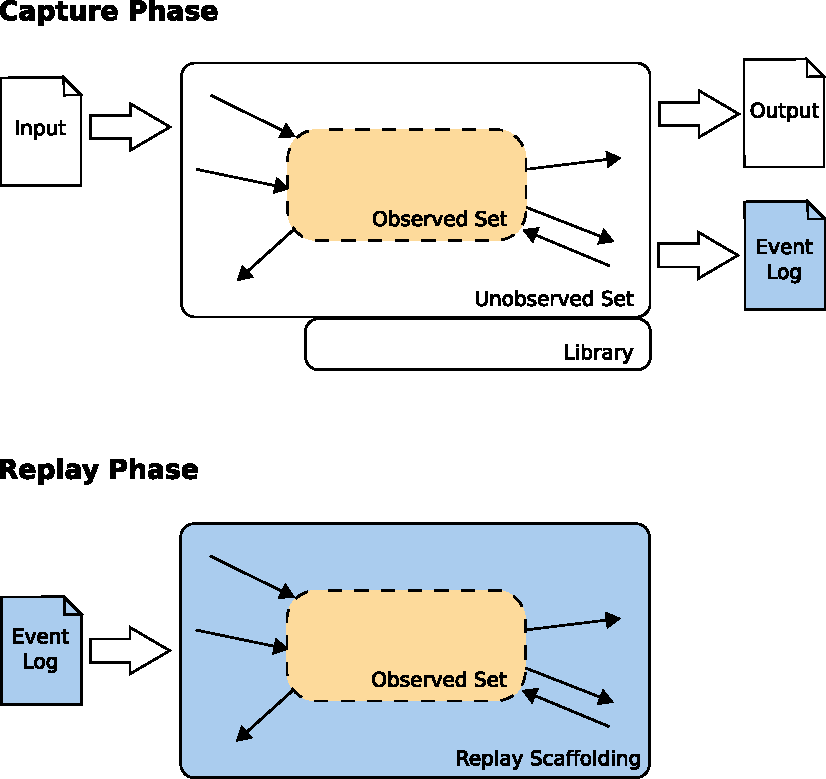
\includegraphics[width=0.8\textwidth]{illustrations/scr_capture_replay_phase}
  \caption{Capture and Replay Phase in Selective Capture and Replay (derived from Joshi and Orso \cite{orso05may})}
  \label{fig:scr_capture_replay_phase}
%\includegraphics{illustrations/capture_and_replay_generic_structure}
\end{figure}
The \emph {capture phase} takes place when the application is run for recording. Before the application starts, the boundaries of the observed set are identified and the application is instrumented in order to be able to capture interactions between the observed set and the rest of the system. While the application runs, the instrumentation generates the events for these interactions and writes them to the \emph{event log}.

In the \emph{replay phase}, the technique generates the \emph{replay scaffolding}. The replay scaffolding uses the event log to replay the events on the observed set. Replaying consists both of performing actions on the observed set (e.g. invocation of a method of the observed set) and consuming actions of the observed set (e.g. receiving a method invocation originally targeted to the unobserved set), thus the replay scaffolding acts both as a driver and stub.

\subsection{Capture Phase}
The capture phase is used to gather the necessary information to replay the application afterwards. In the following we will show how SCARPE \cite{orso05may} gathers that information.

\subsubsection{Capturing Partial Information}
To see the need for a solution of not capturing the whole data that flows over the border clearer, consider the case when a bank tries to find out the time of the last journal entry of an ATM. Assume that the classes \class{BANK} and \class{BANK\_ACCOUNT} belong to the observed set and the rest of the application belongs to the unobserved set. The following instructions access the atm's journal and print the time of the last journal entry:

\javalisting
\begin{lstlisting}
 ATM_JOURNAL journal = atm.journal
 print (journal.time_of_last_entry)
\end{lstlisting}

\class{ATM\_JOURNAL} can contain a thousand of journal entries. In a traditional approach, due to the access to the journal, the whole data structure including all journal entries would be serialized each time the journal is accessed. The idea of selective capture and replay is to only write the referenced object that was passed (the journal) to the event log. When later \class{BANK} accesses the method \texttt{time\_of\_last\_entry}, the result is again written to the event log, because the access crosses the border: from \class{BANK} (observed) to \class{ATM\_JOURNAL} (unobserved). This reduces the size of the event log significantly, because only the the data that is used needs to be written down.

The technique for capturing only partial information instead of the whole data that flows into unobserved set relies on \emph{object IDs}. An object ID uniquely identifies a class instance. SCARPE introduces the object ID into the program by adding an additional field to all modifiable classes. It further instruments the creation constructors of these classes so that the unique object ID is acquired from a global counter. For unmodifiable classes however, a reference map is needed to store the object ID of its instances. The object ID for instances of unmodifiable classes is acquired when it is looked up the first time. The reference map uses weak refences so that the referenced objects can be collected by the garbage collector to avoid memory leaks.

Instead of recursively serializing the data that crosses the boundaries of the observed set, selective capture and replay only records a small part:
\begin{itemize}
 \item Scalar values (values of a basic type) are fully captured.
 \item For objects, the technique only captures the object ID and the type. The type is used to restore the object again during replay phase.
\end{itemize}

Although the rules for this approach are simple, it is not obvious that they suffice to replay an application. Therefore we provide a short reasoning of why this works:

%TODO: bei jedem Punkt 1 Szenario.
\begin{enumerate}
  \item [1)] Instances of observed classes are fully populated during replay, because all actions from the unobserved set are replayed on them and the actions from the observed set are executed on them as in the original run.
  \item [2)] During replay, observed code accesses to methods or fields can either return instances of observed classes or instances of unobserved classes.
  \item [3)] When an object of an observed class is returned, it is fully populated due to 1) and therefore its fields and methods can safely be accessed.
  \item [4)] When an object of an unobserved class is returned, each further access to a field or method from observed code to that object would result in the capturing of another boundary crossing event. Therefore the results of these accesses can be reconstructed during replay.
  \item [5)] Therefore, it is assured that during replay, it is possible for the observed code to access the fields and methods like it did in the original run.
\end{enumerate}



\subsubsection {Interactions between Observed and External Code}
Method calls are an elementary way to communicate between observed and external part of the application. The technique captures calls in both directions: from observed to unobserved code and vice versa. The following events are related to method calls:

%TODO: Beispiel zu jedem event einführen!

\begin{description}
 \item  [OUTCALL] events that represent calls from observed code to unobserved methods.
 \item [INCALL] events that represent calls from unobserved code to observed methods.
 \item [OUTCALLRET] events for the return from outcalls
 \item [INCALLRET] events for the return from incalls
\end{description}

OUTCALL and INCALL events (\emph {call events})  have the same attributes:

\begin{description}
 \item [Receiver] The receiver object
 \item [Method called] Signature of the called method.
 \item [Parameters] The list of scalar values and objects passed to the method.
\end{description}

Capturing of call events involves capturing of scalar values and objects. They are written to the log as follows:

%TODO: log example zeigen:
\begin{description}
 \item [Scalar values] are written verbatim to the log.
 \item [Objects] are written by storing their type and object ID. For null values, the object ID is set to zero. 
\end{description}

OUTCALLRET and INCALLRET events (\emph{callret events}) have only one attribute: the returned value.

OUTCALL and OUTCALLRET events are captured by instrumenting the observed code. A probe is added to all calls to external methods. It is not always possible to distinguish calls to observed code from calls to unobserved code, as we will discuss later.

To capture INCALL and INCALLRET events, proxy methods are introduced in a way that makes it unnecessary to instrument external code. It is ensured that calls inside the observed code don't call these proxy methods but the actual methods. Thus calls from observed code to observed methods can be executed without overhead.

Field Accesses are another source of interaction between observed and external classes. Read accesses from unobserved to observed code don't influence the execution behaviour of the observed code therefore they are not captured. Thus three kinds of events are recorded:

\begin{description}
 \item [OUTREAD] events are generated when observed code reads the content of an unobserved field.
 \item [OUTWRITE] events denote write accesses from observed code to unobserved code.
 \item [INWRITE] events are write accesses from unobserved code to observed code.
\end{description}

OUTREAD, OUTWRITE and INWRITE have the same attributes:

\begin{description}
 \item [Receiver:] The object whose field is accessed.
 \item [Field Name:] The name of the field that is accessed.
 \item [Value:] The read or written value.
\end{description}

OUTREAD and OUTWRITE events are captured by adding probes in the observed code where fields of external classes are accessed. INWRITE events are captured in the same way, but here the unobserved code is instrumented whenever an observed field is written. 

Exceptions are another interaction mechanism that needs to be considered for capture and replay. Because exceptions were not implemented in our Eiffel implementation of selective capture and replay, they will be treated only briefly. For exceptions two more types of events were introduced:
\begin{description}
 \item [EXCIN] events are for exceptions that propagate from the external to the observed code.
 \item [EXCOUT] events are for exceptions that propagate from the internal to the external code.
\end{description}
EXCOUT events are captured by wrapping all observed methods with a \texttt{try-catch} block. By wrapping instructions that call an observed method with an exception handler,  EXCIN events are captured.

\subsection{Replay Phase}
During the replay phase, the observed code is reexecuted based on the event log that was gathered during the capture phase. Before replaying the observed code, selective capture and replay instruments the code based on the interactions between observed and external code. 

\subsubsection{Object Creation}
In the replay phase, object IDs are treated in a different way. Now it is necessary to find the object that matches a given object ID, not reverse. In order to allow this resolving, the technique uses a reference map that maps the object ID to all available  objects. The technique extracts the object IDs from the event's attributes and then retrieves the associated object or creates it. How these objects are created depends on whether they are instances of observed or external classes.
\begin{description}
 \item [Instances of External Classes:] For external classes, \emph{placeholder objects} are created. These objects have the correct type in order to support reflection in the observed code (e.g. \texttt{instanceof}), but their state is irrelevant. After creation, the objects are registered in the reference map.
 \item [Instances of Observed Classes:] Instances of observed objects are either created automatically by the observed code or there must be an INCALL event to the constructor in the event log. When replaying an INCALL to a constructor, an entry for the object is added to the reference map.
 \item [Null Values] If the object ID is zero, \texttt{null} is returned.
\end{description}

\subsubsection{Event Replaying}
For the replay phase, a scaffolding is generated that imitates the behaviour of the external code, thus behaves both as a driver and stub. Whenever control returns to the scaffolding, it checks whether the received event matches the next event in the log. If the events don't match (\emph{out-of-sync events}), a message is displayed to the user, who can chose whether to ignore the discrepacy and continue, or stop the replay.  Out-of-sync events can only occur, if the code was changed between capture and replay phase, for example because the technique is used for regression testing. If the events from log and replay match, the event in the log is  consumed and replay continues. Otherwise the technique asks the user whether he wants to abort or skip the unmatched event and continue.

In contrast to INCALL, INWRITE, OUTREAD, OUTCALLRET and EXCIN, which are necessary to replay the observed code correctly, OUTCALL, INCALLRET, OUTWRITE, EXCOUT are not necessary to replay the observed code, but they can be used as oracles for regression testing. The observed set is considered to be the system under test, which generates OUTCALLL, INCALLRET, OUTWRITE and EXCOUT events as output, these events can then be compared to the recorded events of the capture phase - the recorded events are used as oracle.

\begin{description}
%TODO: example einweben!
 \item [INCALL Events] To replay INCALL events, the method first retrieves the target object from the reference map. If the target object is not in the reference map, it must be either a call to a constructor or a static call. Then, it retrieves the parameters from the reference map, or creates the scalar values corresponding to the parameters. If the object can't be retrieved from the reference map, a placeholder object is created. Then, the technique can call the specified method with all arguments; the control flows to the observed code. 
 \item [INCALLRET Events] INCALLRET events are not essential for replaying the observed code. They occur as a result of INCALL events and are consumed by the replay scaffolding. To ensure a correct replay, the scaffolding checks if returned value conforms to the one of the next event in the event log.
 \item [OUTCALL Events] All invocations to unobserved methods from the observed code are replaced by two instructions: (1) The call to a special feature in the scaffolding (\texttt{consumeCall}) and (2) The assignment of the result of the invocation. For example \texttt{TIME t = atm\_journal.time\_of\_last\_entry()}, with TIME and ATM\_JOURNAL both being in the package \texttt{foo}, would be replaced by the following instructions:
\begin{lstlisting}
 Object tmp = scaffolding.consumeCall("foo/ATM_JOURNAL",
                24,/*object ID for atm_journal*/
                "time:()Lfoo/TIME",
                {} /*empty array of parameters*/
		);
 TIME t = (TIME) tmp;
\end{lstlisting}
The scaffolding checks whether type, parameters, target and methodname of the next event from the log matches to the reported call. If the events match, then replay continues with the next event, otherwise an error is reported to the user.
 \item [OUTCALLRET Events]As these events occur as a result of OUTCALL events, they are treated within \texttt{consumeCall}. The method looks up the return value in the event log and retrieves it using the reference map. 
 \item [OUTREAD and OUTWRITE Events] To replay these events, accesses to unobserved fields are instrumented in the observed code, by calling associated methods from the scaffolding, \texttt{consumeRead} for OUTREAD events and \texttt{consumeWrite} for OUTWRITE events. For example the instruction \texttt{ATM\_JOURNAL journal = atm.journal}, with ATM\_JOURNAL and ATM both belonging to package \texttt{foo}, would be replaced by the following instruction:
\begin{lstlisting}
 ATM_JOURNAL journal = scaffolding.consumeRead ("foo/ATM",
                24,/*Object ID for atm*/
                "val")
\end{lstlisting}
The methods \texttt{consumeRead} and \texttt{consumeWrite} check if the event from the log matches the detected one. The method \texttt{outRead} furthermore returns value associated with the event.
 \item [INWRITE Events] In order to replay an INWRITE event, the scaffolding retrieves the target, the name of the field that should be modified and the value to be assigned. It resolves the target, which must exist unless it is a static field access. The value to be assigned is resolved as well or created if it does not exist yet. Finally the scaffolding sets the field of the target to the specified value.
 \item [EXCIN and EXCOUT Events]  To replay EXCIN events, the method \texttt{consumeCall} creates and throws a corresponding exception. This is possible, because EXCIN events can only occur during an outcall. EXCOUT events, which are generated by the observed code, are caught by the replay scaffolding and compared to the next event in the event log. If the exception matches the event from the event log, replay continues.
\end{description}

\subsubsection{Assumptions}
The following list of assumption are required for selective capture and replay:
\begin{itemize}
 \item It is assumed that there is no direct access from unmodifiable classes to fields of observed classes.
 \item Because native code is not instrumented, Joshi and Orso also assume that there is no direct access from native code to observed fields.
 \item The technique can not guarantee the same thread schedule during capture and replay phase. Therefore it is assumed that the interleaving due to multi-threading does not change the behaviour of the observed code.
 \item The technique assumes that runtime exceptions occur deterministically. This is necessary, because exceptions generated in the observed code are consumed, but not replayed.
\end{itemize}

\subsubsection{Special Cases}
There are some special cases that need to be considered when implementing selective capture and replay:

%TODO: Beispiele einfüge!
\begin{description}
 \item [Polymorphism and Dynamic Binding] It is not always possible to determine whether an event is internal or external, when it depends on the dynamic type of the receiver. In these cases, it is necessary to add a runtime check to determine whether the receiver is an internal or external class, which is done using the \texttt{instanceof} operator. \texttt{XXX Is this insertion here valid?} We assume that this case occurs at least in examples that use multiple interface inheritance, where it can not be assumed that the implementors of an interface are either all in the observed set or all in the unobserved set.
 \item [Inheritance] If a class \emph{c} is in the observed set, but not all of \emph{c's} subclasses, creating an instance of any of \emph{c's} subclasses would result in the creation of an instance of \emph{c}. To avoid this issue, it is required that if a class \emph{c} is added to the observed set, all subclasses of \emph{c} are also in the observed set. We assume that problem described here is implementation specific, and could be avoided.
 \item [Reflection] The technique handles most cases of reflection, however in some cases, additional instrumentation is required (e.g. if reflection is used in external code to modify fields of observed classes). 
 \item [Access Modifiers] In order to replay recorded executions, in some cases it is necessary to change access modifiers. We assume that this applies primarily to the \texttt{protected} modifier, which may prohibit access to observed classes from within the replay scaffolding.
 \item [Garbage Collection] To allow the collection of unused objects, the technique must make sure that it does not keep references to unused objects. For example the reference map must use weak references to avoid memory leaks.
 \item [Finalize] Calls to \texttt{finalize} are non-deterministic in Java, thus they can generate out-of-sync events during the replay phase. Therefore calls to \texttt{finalize} are treated in a special way: when receiving a call to \texttt{finalize}, the technique consumes the next matching entry in the event log, that is a call to \texttt{finalize}.
\end{description}

%-Eiffel compilation model (?)
%-CDD (?)
\chapter{Capture and Replay for Eiffel}
\eiffellisting
\section{Differences to Existing Implementation}
Selective capture and replay as described by Joshi and Orso \cite{orso05may} can not be directly applied to Eiffel. Although the core elements of the technique can be used in Eiffel, too, we need to adapt some parts. In this section the changes to the original implementation and reasons for these changes will be discussed.

\subsection{Language Aspects}
Even though Java and Eiffel are both object oriented languages, there are differences between these two languages, syntax left aside. Eiffel offers a wider set of language constructs, many times trying to solve problems inherently object oriented, whereas Java reused solutions from its ancestors, mainly C++. One example for this difference could be the Eiffel basic types, which can be treated as objects with methods and attributes versus the Java basic types, which are no objects. This section focuses on the differences between Java and Eiffel that influenced our implementation of selective capture and replay.

\subsubsection{Terminology} % diesen Titel weglassen?
Eiffel has a nomenclature that differs from other programming languages. Here the Eiffel terminology is described according to \cite{oosc2} and compared to the one from Java.
\begin{center}
\begin{tabular}[]{|l|l|} \hline
 \textbf{Eiffel}&\textbf{Java} \\ \hline
 Attribute&Field \\ \hline
 Ouery&Field or Method that has a return value \\ \hline
 Routine&Method \\ \hline
 Procedure&Method that has no return value \\ \hline
 Function&Method that has a return value \\ \hline
 Feature&Method or Attribute \\ \hline
 ANY&Object (ancestor of all classes) \\ \hline
\end{tabular} 
\end{center}

\subsubsection{Multiple Inheritance}
Eiffel is designed to support multiple inheritance, whereas in Java, only single inheritance is allowed. The original implementation assumes, that all subclasses of a class \emph{c} are in the observed set iff \emph{c} is also in the observed set. This makes it possible to statically decide whether an observed or an unobserved feature is accessed.

If this assumption is translated to multiple inheritance, it would not be possible to have a class \emph{C} that inherits both from an observed class \emph{A} and an unobserved class \emph{B} (\figref{fig:obs_unobs_multiple_inheritance}).
\begin{figure}[ht]
  \centering
  
\includegraphics[width=0.5\textwidth]{illustrations/obs_unobs_multiple_inheritance}
  \caption{Conflict Due to Multiple Inheritance}
  \label{fig:obs_unobs_multiple_inheritance}
%\includegraphics{illustrations/capture_and_replay_generic_structure}
\end{figure}

Multiple inheritance is extensively used in Eiffel, thus this assumption would be too restrictive in our opinion. It would lead to big clusters that could not be divided into observed and unobserved set. 

Although Java does not allow multiple inheritance, it supports multiple interface inheritance. Joshi and Orso \cite{orso05may} mention that they need to dynamically determine if the target of an event is observed or unobserved in certain cases. We assume that multiple interface inheritance with a class that both implements an observed and unobserved interface  is at least one of these cases. They use the \texttt{instanceof} operator determine if an object is an instance of an observed class.

We will present a solution that always determines dynamically, if an object is an instance of an observed class (\emph{observed object}) or an instance of an unobserved class (\emph{unobserved object}), together with a proposal how to solve this problem without reflection.

\subsubsection{Read Only Attributes}
Eiffel strictly follows the \emph{uniform access principle} \cite{oosc2}. The principle states that it should not be visible to the clients whether features are implemented through storage or computation. This ensures that the implementation of a feature could be changed from attribute to function or vice versa. One of the consequences of this principle is that clients of a class cannot write to attributes, as these attributes could be implemented as a function as well.

In Java, this principle is not ensured because clients of a class can write to their fields. For our implementation of selective capture and replay, this limits the events related to field accesses to OUTREAD. Both OUTWRITE and INWRITE can not happen, because write access to fields is restricted to their class, thus there can not be any write accesses to fields from observed to unobserved classes or reverse.

\subsection{Target Application}
As a first application that could use selective capture and replay in Eiffel, Cdd, a tool for Contract Driven Development \cite{cdd07} was chosen. Cdd allows programmers to extract test cases from failing program runs. The contracts that are present in the code are used as test oracles.Cdd is not always able to generate such a test case, due to different reasons:

\begin{description}
\item [Prestate extraction:] The state before calling the failing feature (which is needed to generate a test case) is extracted using the state at the time of failure. Because not all instructions between feature call and failure can be undone, the extraction of the prestate is not always possible.
\item [Non-determinism:] If the failing feature reads values from sources that don't always return the same values (eg. user input), it's not generally possible to run the test cases with the same result as in the failing run.
\item [External state:] When the feature relies on state that is not stored in Eiffel objects (e.g. in C structs), Cdd is not able to gather this state for the test.
\end{description}

All these limitations can be resolved using selective capture and replay:
\begin{description}
\item [Prestate extraction:] By setting a breakpoint at the beginning of the failing feature, it is possible to extract the prestate during the replay of the application.
\item [Non-determinism:] When adding all non-deterministic classes to the unobserved set, it can be ensured that the replay of the run is deterministic.
\item [External State:] All classes that wrap external state can be added to the unobserved set. Thus interactions with these classes can be replayed without having to store the external state.
\end{description}

Prestate extraction using selective capture and replay requires an immediate rerun of the application under test. Because complete recompiles in Eiffel last for tens of minutes up to hours, we can not afford to instrument the application again before replaying it. Thus it is necessary to design the code instrumentation to be both applicable for capture and replay phase. We pushed this approach even further to allow the user to disable the whole instrumentation. This allows execution with minimal overhead if capture and replay is not needed without recompiling the application.

\section{Code Instrumentation}
\subsection{Outline}
Due to differences between Eiffel and Java and a different use case, there are two main differences between the original implementation and our approach:

\begin{enumerate}
 \item It is necessary to determine dynamically whether an object is observed or not.
\item It must be possible to switch between capture and replay phase without reinstrumenting the code.
\end{enumerate}

The first requirement can be met by adding an additional query to every class so that it is possible to find out whether an object is an instance of an observed or an unobserved class. We ensure that every class has this query by adding it to ANY. In the next chapter we will discuss how this query can be implemented efficiently.

In order to be able to switch between capture and replay mode, the class PROGRAM\_FLOW\_SINK was introduced. Program flow events are put into the PROGRAM\_FLOW\_SINK. It is both the ancestor class of RECORDER, the class that contains the management code for recording events and PLAYER, the class that provides the scaffolding for replaying events. The standard instance of a PROGRAM\_FLOW\_SINK is globally accessible. It is dynamically bound to an instance of RECORDER during capture phase and PLAYER during replay phase.

To create placeholder objects from unobserved classes, their original routine bodies are disabled during replay pha phase. When replaying, the routines only execute instrumentation code that invokes the scaffolding and takes care of the return value if necessary.

\subsection{Routines}
Whereas the original implementation captures routine calls by instrumenting the call site (in the client), we decided to instrument the calee (the supplier). This simplifies code instrumentation, because there is no need to make changes inside existing routine bodies, it is sufficient to add some code at the beginning and the end of the routine bodies. %TODO Gibt es noch ein besseres Motiv?

The routine instrumentation can be divided into three parts (\figref{fig:routine_instrumentation_structure}): Right at the beginning of the routine, code to detect call events is inserted. The original routine body is made conditional so that it is not executed for unobserved routines during the replay phase. Finally, code to detect callret events is inserted at the end of the routine.
\begin{figure}[ht]
  \centering
  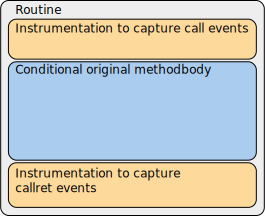
\includegraphics[width=0.5\textwidth]{illustrations/routine_instrumentation_structure}
  \caption{Structure of Routine Instrumentations}
  \label{fig:routine_instrumentation_structure}
\end{figure}

To explain instrumentation in more detail, we describe each of these three parts using the command \texttt{withdraw} of the class \texttt{ATM} (\listref{lst:account_exists_original}).

\begin{lstlisting}[caption=Original Code of Command \texttt{withdraw} ,label=lst:account_exists_original]
account_exists (account_name:STRING): BOOLEAN
		-- Is there an account with name 'account_name'?
	require
			account_name_not_void: account_name /= Void
	do
		Result := (the_bank.account_for_name (account_name) /= Void)
	end
\end{lstlisting}

\subsubsection{Capturing Call Events}
To capture call events, instrumented code, which is only executed when capture and replay is enabled, is inserted at the beginning of every routine. The code first detects whether the routine was called across the boundaries. If that is the case, it puts the associated event into the program flow \listref{lst:invocation_instrumentation}
\begin{lstlisting}[caption=Instrumentation Code to Detect Call Events,label=lst:invocation_instrumentation]
if program_flow_sink.is_capture_replay_enabled then
	program_flow_sink.enter
	if program_flow_sink.observed_stack_item /= is_observed then
		program_flow_sink.put_to_observed_stack (is_observed)
		program_flow_sink.put_feature_invocation ("account_exists", Current, [account_name])
	else
		program_flow_sink.put_to_observed_stack (is_observed)
	end
	program_flow_sink.leave
end
\end{lstlisting}
Note that all the inserted code is part of the selective capture and replay management code, which does not belong to the code of the original application. Thus these instructions must not trigger further events for the event log (e.g. the creation of the manifest string ``withdraw'' should not create other call events on class STRING). To make sure, that this won't happen, the commands \texttt{enter} to disable capture and replay and \texttt{leave} to reenable capture and replay were implemented.

To detect boundary crossing calls, the management code keeps an own stack that indicates whether the target objects of the calls on the call stack are observed or not. This stack is managed in parallel to the call stack; in the invocation instrumentation code, the result of the query \texttt{is\_observed} is put onto the stack and in the exit instrumentation code, thes value is removed again. Using this stack, it is possible to find out, whether the caller object was observed or not.
\subsubsection{Conditional Routine Body Execution}
To be able to switch between the original and the placeholder routine body, the original routine of unobserved routines is only executed during capture phase. Placeholder routines are only needed for unobserved routines, thus the original body is always executed for observed routines (\listref{lst:methodbody_instrumentation}). The query \texttt{is\_replay\_phase} always returns false, when capture and replay is disabled, therefore the management code will always use the original routine body.

\begin{lstlisting}[caption=Conditional Methodbody,label=lst:methodbody_instrumentation]
if (not program_flow_sink.is_replay_phase) or is_observed then
	Result := (the_bank.account_for_name (account_name) /= Void)
end
\end{lstlisting}
\subsubsection{Capturing Callret Events}
To capture and replay callret events, instrumentation code is inserted at the end of the routines. Again, the code only puts an event into the \texttt{program\_flow\_sink} if the routine was called across the boundary. If the routine is a function, the code also restores the result that was computed in the capture phase for unobserved functions. The result is only restored for unobserved classes during replay phase, otherwise the query \texttt{last\_result} returns the same value that was put into the \texttt{program\_flow\_sink} before. Thus functions can be used as placeholder functions without altering the instrumentation between capture and replay phase.
\begin{lstlisting}[caption=Instrumentation to Capture Callret Events,label=lst:exit_instrumentation]
if program_flow_sink.is_capture_replay_enabled then
	program_flow_sink.enter
	program_flow_sink.remove_from_observed_stack
	if program_flow_sink.observed_stack_item /= is_observed then
		program_flow_sink.put_feature_exit (Result)
		Result ?= program_flow_sink.last_result
	end
	program_flow_sink.leave
end
\end{lstlisting}

\subsubsection{Complete Routine Instrumentation}
\listref{lst:account_exists_instrumented} shows the routine after combining all three parts of the instrumentation.
\begin{lstlisting}[caption=Routine \texttt{account\_exists} After Instrumentation,label=lst:account_exists_instrumented]
account_exists (account_name: STRING_8): BOOLEAN
		-- Is there an account with name 'account_name'?
	require
		account_name_not_void: account_name /= Void
	do
		if program_flow_sink.is_capture_replay_enabled then
			program_flow_sink.enter
			if program_flow_sink.observed_stack_item /= is_observed then
				program_flow_sink.put_to_observed_stack (is_observed)
				program_flow_sink.put_feature_invocation ("account_exists", Current, [account_name])
			else
				program_flow_sink.put_to_observed_stack (is_observed)
			end
			program_flow_sink.leave
		end
		if (not program_flow_sink.is_replay_phase) or is_observed then
			Result := (the_bank.account_for_name (account_name) /= Void)
		end
		if program_flow_sink.is_capture_replay_enabled then
			program_flow_sink.enter
			program_flow_sink.remove_from_observed_stack
			if program_flow_sink.observed_stack_item /= is_observed then
				program_flow_sink.put_feature_exit (Result)
				Result ?= program_flow_sink.last_result
			end
			program_flow_sink.leave
		end
	end
\end{lstlisting}

\subsection{Attribute Accesses}
\texttt{TODO!!!}

\subsection{Attribute Manipulation from C Level}
One assumption of the original selective capture and replay implementation is that native code never manipulates observed fields. Eiffel allows integration of C code into classes, using the \texttt{external} keyword. In order to write to fields of Eiffel objects, the C code needs the adress of that object, which can be done using the \texttt{\$} - operator.

To find out the classes whose fields are written from native code, we searched for the \texttt{\$} operator in the Eiffel base library. Writes to \texttt{{STRING}.area} of type \texttt{SPECIAL [CHARACTER]} (where the characters of strings are stored) is most common and needed to be adressed. 

this would be too restrictive. On the other hand, it is not possible to automatically instrument the integrated C code, therefore we require manual instrumentation when attributes are written from native code.


\section{Architecture}
%unterschiedliche Parts noch genauer beschreiben
%-Log: (mikro-architektur), wieso kein XML?
\section{Advantages over Traditional Capture and Replay}
\section{Limitations}
%unter welchen Umstaenden musste manuell instrumentiert werden??
\section{Future Steps}
%Fehlende features + idee zu deren implementierung

\section{Building the Example from Source}
In this section the process of building an example with capture replay support under Linux will be described. Setting up the modified version of Eiffel Studio and all necessary tools will take the biggest part of this explanation.\\
%TODO: wieso genau wird eine modifizierte Version von Eiffel Studio benoetigt??
It is assumed that all commands in the following steps are executed in the same session, thus keeping the environment variables.\\

\subsection{Building the Preliminaries}
The first tools we need are the  Eiffel Studio Tools \cite{estudiotools}. These will be used in many setup scripts in the examples or tests from the repository. Install those tools according to the description on the webpage.\\

The delivery of the modified Eiffel Studio was built using revision 69201 of Eiffel Studio. Building a delivery with a later version of Eiffel Studio was not testet, so it might not work. If no binaries of revision 69201 are available, a delivery of that revision from source \texttt{(stimmt das wirklich??? gaebe das kein Henne / Ei Problem?)}.\\
After copying the delivery to ~/estudio/Eiffel60\_gpl\_69201, it can be activated:
\bashlisting
\begin{lstlisting}
   activate_estudio 60_gpl_69201
\end{lstlisting}

Now Gobo \cite{gobo} can be installed can be installed from svn (Revision 6001 was successfully tested).
- Install Gobo  from svn (revision 6001) -->
\begin{lstlisting}
svn co -r6001 https://gobo-eiffel.svn.sourceforge.net/svnroot/gobo-eiffel/gobo/trunk ~/capture_replay/gobo
export GOBO=~/capture\_replay/gobo
export PATH=$GOBO/bin:$PATH
$GOBO/work/bootstrap/bootstrap.sh gcc ise
\end{lstlisting}

As all preliminaries are installed, Erl-G \cite{erlg} can be downloaded and built. Revision 719 of Erl-G was tested together with capture and replay.
\begin{lstlisting}
svn co -r719 https://svn.origo.ethz.ch/autotest/trunk/erl_g ~/capture_replay/erl_g
export ERL_G=~/capture_replay/erl_g
export PATH=$ERL_G/bin:$PATH
cd $ERL_G
#EIFFEL_SRC is needed. avoid conflicts between EIFFEL_SRC and ISE_LIBRARY.
export ISE_LIBRARY=$EIFFEL_SRC
geant install
geant compile
\title{Selective Capture and Replay for Eiffel
\end{lstlisting}

To build a delivery of the modified Eiffel Studio, execute these commands: (this will take a few hours).
\begin{lstlisting}
cd ~/capture_replay/
mkdir es
svn co https://eiffelsoftware.origo.ethz.ch/svn/es/branches/capture_replay es
export EIFFEL_SRC=~/capture_replay/es/Src
cd es
geant -b $EIFFEL_SRC/scripts/build.eant build_es
\end{lstlisting}

Before an example can be built the delivery that was just created needs to used be set as default instance of Eiffel Studio
\begin{lstlisting}
cd ~/estudio
ln -s ~/capture_replay/es/EiffelXX EiffelCR
activate_estudio CR
\end{lstlisting}

In order to make the created Eiffel Studio use a modified version of the runtime, it is necessary to recompile the runtime with modified CFLAGS. The new version of the runtime then needs to be installed in the delivery.

It is not possible to directly build Eiffel Studio with the modified version of the runtime, because the changes in the runtime are not compatible to Eiffels store mechanism (\texttt{TODO: das auch noch unter irgendwelchem future work anmerken...}). This would render Eiffel Studio unusable because it relies on this mechanism during the build process.
\begin{lstlisting}
export CFLAGS='-DCAPTURE_REPLAY' 
cd $EIFFEL_SRC
#build the runtime from scratch (clobber the old one)
geant -b scripts/build.eant compile_runtime
cd $ISE_EIFFEL/studio/spec/linux-x86/lib
rm *
cp $EIFFEL_SRC/C/run-time/lib* .
\end{lstlisting}


\subsection{Building an Example}
Now, all necessary tools should be installed and the corresponding environment variables set. And we can start to build an example.\\
First we need to add reflection support to the example project. Erl G will generate reflection classes for us. If the environment variables are correctly set, the geant script should invoke Erl G automatically. \\
At the moment Erl-G does not support overrides because this feature is missing in the Gobo parser. Therefore it's necessary to override the necessary classes manually. There are two geant tasks that take care of this:

\begin{itemize}
\item \identifier{patch\_elks} makes the manual override by copying the modified elks classes from \$EIFFEL\_SRC/library/base/capture\_replay/elks\_overrides to \$ISE\_LIBRARY/library/base/elks \\
\item \identifier{unpatch\_elks} restores the original state by copying the original elks classes from \$EIFFEL\_SRC/library/base/elks to \$ISE\_LIBRARY/library/base/elks .
\end{itemize}

\begin{lstlisting}
cd ~/capture_replay/es/examples/capture_replay/iteration1
geant install
\end{lstlisting}

The example can now be opened with the modified version of Eiffel Studio. Make sure that the CFLAGS are still set to '-DCAPTURE\_REPLAY'. Otherwise it will not be possible to build the example.



\section {Limitations}
%-Konstruktoren nach ANY exportiert (fehlende unterstuetzung von Eiffel-Seite fuer Konstruktoren)
%- Access modifiers e.g. export of a observed feature only to an unobserved class --> replay not possible.

% Unterschiedliche Language features Eiffel/Java
% Unterschiede der Anforderungen
% -keine dynamische Kompilierung
%  capture/replay ohne neukompilierung (cdd)

\chapter{Implementation}
\section{Architecture}
%unterschiedliche Parts noch genauer beschreiben
%-Log: (mikro-architektur), wieso kein XML?
\section{Code Instrumentation}
\subsection{Procedures}
\subsection{Direct Manipulation from C Level}
\subsection{Field Accesses}
\section{Advantages over Traditional Capture and Replay}
\section{Limitations}
%unter welchen Umstaenden musste manuell instrumentiert werden??
\section{Future Steps}
%Design des Management Codes
% Idee der Instrumentierung & Beispiel
% Vorteile gegenüber der Original Implementierung
% Limitations
% Experimental Results
\section{Building the Example from Source}
In this section the process of building an example with capture replay support under Linux will be described. Setting up the modified version of Eiffel Studio and all necessary tools will take the biggest part of this explanation.\\
%TODO: wieso genau wird eine modifizierte Version von Eiffel Studio benoetigt??
It is assumed that all commands in the following steps are executed in the same session, thus keeping the environment variables.\\

\subsection{Building the Preliminaries}
The first tools we need are the  Eiffel Studio Tools \cite{estudiotools}. These will be used in many setup scripts in the examples or tests from the repository. Install those tools according to the description on the webpage.\\

The delivery of the modified Eiffel Studio was built using revision 69201 of Eiffel Studio. Building a delivery with a later version of Eiffel Studio was not testet, so it might not work. If no binaries of revision 69201 are available, a delivery of that revision from source \texttt{(stimmt das wirklich??? gaebe das kein Henne / Ei Problem?)}.\\
After copying the delivery to ~/estudio/Eiffel60\_gpl\_69201, it can be activated:
\bashlisting
\begin{lstlisting}
   activate_estudio 60_gpl_69201
\end{lstlisting}

Now Gobo \cite{gobo} can be installed can be installed from svn (Revision 6001 was successfully tested).
- Install Gobo  from svn (revision 6001) -->
\begin{lstlisting}
svn co -r6001 https://gobo-eiffel.svn.sourceforge.net/svnroot/gobo-eiffel/gobo/trunk ~/capture_replay/gobo
export GOBO=~/capture\_replay/gobo
export PATH=$GOBO/bin:$PATH
$GOBO/work/bootstrap/bootstrap.sh gcc ise
\end{lstlisting}

As all preliminaries are installed, Erl-G \cite{erlg} can be downloaded and built. Revision 719 of Erl-G was tested together with capture and replay.
\begin{lstlisting}
svn co -r719 https://svn.origo.ethz.ch/autotest/trunk/erl_g ~/capture_replay/erl_g
export ERL_G=~/capture_replay/erl_g
export PATH=$ERL_G/bin:$PATH
cd $ERL_G
#EIFFEL_SRC is needed. avoid conflicts between EIFFEL_SRC and ISE_LIBRARY.
export ISE_LIBRARY=$EIFFEL_SRC
geant install
geant compile
\title{Selective Capture and Replay for Eiffel
\end{lstlisting}

To build a delivery of the modified Eiffel Studio, execute these commands: (this will take a few hours).
\begin{lstlisting}
cd ~/capture_replay/
mkdir es
svn co https://eiffelsoftware.origo.ethz.ch/svn/es/branches/capture_replay es
export EIFFEL_SRC=~/capture_replay/es/Src
cd es
geant -b $EIFFEL_SRC/scripts/build.eant build_es
\end{lstlisting}

Before an example can be built the delivery that was just created needs to used be set as default instance of Eiffel Studio
\begin{lstlisting}
cd ~/estudio
ln -s ~/capture_replay/es/EiffelXX EiffelCR
activate_estudio CR
\end{lstlisting}

In order to make the created Eiffel Studio use a modified version of the runtime, it is necessary to recompile the runtime with modified CFLAGS. The new version of the runtime then needs to be installed in the delivery.

It is not possible to directly build Eiffel Studio with the modified version of the runtime, because the changes in the runtime are not compatible to Eiffels store mechanism (\texttt{TODO: das auch noch unter irgendwelchem future work anmerken...}). This would render Eiffel Studio unusable because it relies on this mechanism during the build process.
\begin{lstlisting}
export CFLAGS='-DCAPTURE_REPLAY' 
cd $EIFFEL_SRC
#build the runtime from scratch (clobber the old one)
geant -b scripts/build.eant compile_runtime
cd $ISE_EIFFEL/studio/spec/linux-x86/lib
rm *
cp $EIFFEL_SRC/C/run-time/lib* .
\end{lstlisting}


\subsection{Building an Example}
Now, all necessary tools should be installed and the corresponding environment variables set. And we can start to build an example.\\
First we need to add reflection support to the example project. Erl G will generate reflection classes for us. If the environment variables are correctly set, the geant script should invoke Erl G automatically. \\
At the moment Erl-G does not support overrides because this feature is missing in the Gobo parser. Therefore it's necessary to override the necessary classes manually. There are two geant tasks that take care of this:

\begin{itemize}
\item \identifier{patch\_elks} makes the manual override by copying the modified elks classes from \$EIFFEL\_SRC/library/base/capture\_replay/elks\_overrides to \$ISE\_LIBRARY/library/base/elks \\
\item \identifier{unpatch\_elks} restores the original state by copying the original elks classes from \$EIFFEL\_SRC/library/base/elks to \$ISE\_LIBRARY/library/base/elks .
\end{itemize}

\begin{lstlisting}
cd ~/capture_replay/es/examples/capture_replay/iteration1
geant install
\end{lstlisting}

The example can now be opened with the modified version of Eiffel Studio. Make sure that the CFLAGS are still set to '-DCAPTURE\_REPLAY'. Otherwise it will not be possible to build the example.

\chapter{Experimental Results}
\section{Example Application}
\section{Results}
\section{Conclusion}
%Eiffel Vision Beispiel, mit unterschiedlichen observed sets

\chapter{Future Work}
%Fehlende C/R und Language Features beschreiben, sowie einen möglichen Lösungsansatz.
\chapter{Appendix}

\subsection{Log File Grammar}

log ::= event* \\
event ::= call $\mid$ return $\mid$ outread\\
call ::= calltype entity methodname entity* \texttt{“\%N”} \\
return ::= returntype [entity]  \texttt{“\%N”}\\
outread ::= \texttt{OUTREAD} entity attribute\_name entity
calltype ::= \texttt{INCALL} $\mid$ \texttt{OUTCALL} \\
returntype ::= \texttt{INCALLRET} $\mid$ \texttt{OUTCALLRET} \\
methodname ::= identifier \\
attribute\_name ::= identifier \\
entity ::= (object $\mid$ value) \\
size ::= integer \\
object ::= \texttt{[NON$\_$BASIC} typename object\_id \texttt{]} \\
value ::= \texttt{[BASIC} typename \texttt{"} string \texttt{"]} \\
typename ::= identifier \\
object\_id ::= integer\\
identifier ::= [A-Za-z]character*\\
string ::= character*\\

\subsection{capture-phase performance measurements}
\begin{itemize}
	\item normal application: 2.5s
	\item Captured application: 30s
	\begin{itemize}
		\item RECORDER: 1.7s\\
		\item SERIALIZER: 26s
		\begin{itemize}
			\item write$\_$statements: 16s
			\begin{itemize}
				\item file.put$\_$string: 4s
				\item object$\_$id: 7s
				\item other: 5s
			\end{itemize}
			\item is$\_$basic$\_$type: 3s
			\item other: 7s
		\end{itemize}
	\end{itemize}
\end{itemize}

\bibliographystyle{plain} 
\bibliography{thesis}

\end{document}


